\documentclass[a4paper,UTF8]{article}
\usepackage{ctex}
\usepackage[margin=1.25in]{geometry}
\usepackage{color}
\usepackage{graphicx}
\usepackage{amssymb}
\usepackage{amsmath}
\usepackage{amsthm}
\usepackage{soul, color, xcolor}
\usepackage{bm}
\usepackage{tcolorbox}
\usepackage{hyperref}
\numberwithin{equation}{section}
%\usepackage[thmmarks, amsmath, thref]{ntheorem}
\theoremstyle{definition}
\newtheorem*{solution}{Solution}
\newtheorem*{prove}{Proof}
\usepackage{multirow}
\usepackage{diagbox}
\usepackage{float}

\def \X {\boldsymbol{X}}
\def \Y {\boldsymbol{Y}}
\def \A {\boldsymbol{A}}
\def \w {\boldsymbol{w}}
\def \u {\boldsymbol{u}}
\def \v {\boldsymbol{v}}
\def \s {\boldsymbol{s}}
\def \y {\boldsymbol{y}}
\def \x {\boldsymbol{x}}
\def \z {\boldsymbol{z}}
\def \hy {\widehat{y}}
\def \by {\Bar{y}}
\def \H {\mathbf{H}}
\def \I {\mathbf{I}}
\def \boldalpha {\boldsymbol{\alpha}}
\def \boldbeta {\boldsymbol{\beta}}
\def \bdalpha {\boldsymbol{\alpha}}
\def \bdbeta {\boldsymbol{\beta}}
\def \bdxi {\boldsymbol{\xi}}
\def \bdepsilon {\boldsymbol{\epsilon}}
\newcommand\given[1][]{\:#1\vert\:}
\setlength{\parindent}{0pt}
%--

%--
\begin{document}
\title{机器学习导论\ 习题三}
\author{211300044, 吴羽珩, \href{mailto:邮箱}{211300044@smail.nju.edu.cn}}
\maketitle
\section*{作业提交注意事项}
\begin{tcolorbox}
	\begin{enumerate}
		\item[1.] 请在LaTeX模板中第一页填写个人的学号、姓名、邮箱;
		\item[2.] 本次作业需提交作答后的该 pdf 文件、编程题代码(.py文件); {\color{red}\textbf{请将二者打包为~.zip 文件上传}}. 注意命名规则, 三个文件均命名为 “$\text{学号}\_\text{姓名}$” + “$.\text{后缀}$” (例如“$\text{211300001}\_\text{张三}$” + “.pdf”、“.py”、“.zip”);
		\item[3.] 若多次提交作业, 则在命名~.zip 文件时加上版本号, 例如“211300001\_张三\_v1.zip” (批改时以版本号最高的文件为准);
		\item[4.] 本次作业提交截止时间为 {\color{red}\textbf{ 5 月 2 日23:59:59}}. 未按照要求提交作业, 提交作业格式不正确, {\color{red}\textbf{作业命名不规范}}, 将会被扣除部分作业分数; 除特殊原因 (如因病缓交, 需出示医院假条) 逾期未交作业, 本次作业记 0 分; {\color{red}\textbf{如发现抄袭, 抄袭和被抄袭双方成绩全部取消}};
		\item[5.] 本次作业提交地址为 \href{https://box.nju.edu.cn/u/d/71102ced9a9b4d6f8d05/}{here}, 请大家预留时间提前上交, 以防在临近截止日期时, 因网络等原因无法按时提交作业.
	\end{enumerate}
\end{tcolorbox}
\newpage

\section{[20pts] Representor Theorem}
表示定理告诉我们, 对于一般的损失函数和正则化项,优化问题的最优解都可以表示为核函数的线性组合. 我们将尝试证明表示定理的简化版本, 
并在一个实际例子中对其进行应用. 请仔细阅读《机器学习》第六章6.6节, 并回答如下问题.
\begin{enumerate}
    \item[(1)] \textbf{[10pts]} 考虑通过引入核函数来将线性学习器拓展为非线性学习器, 优化目标由结构风险和经验风险组成:
    \begin{align*}
        \min_{\w} \  J(\w) = \frac{1}{m} \sum_{i=1}^m \mathcal{L}\left(\w^T \phi(\x_i), y_i \right) + \frac{\lambda}{2}\|\w\|^2,
    \end{align*}
    其中映射$\phi: \mathcal{X} \to \mathbb{H}$将样本映射到特征空间$\mathbb{H}$, $\mathcal{L}$为常见的损失函数,
    并记$\X = \left[\phi(\x_1), \cdots, \phi(\x_m)\right]$为映射后的数据矩阵. 请证明: 优化问题的最优解$\w^\star$属于矩阵$\X$的列空间, 即$\w^\star \in \mathcal{C}(\X)$.

    (提示: 给定线性子空间$\mathcal{S}$, 任意向量$\u$有唯一的正交分解$\u = \v + \s(\v \in \mathcal{S}, \s \in \mathcal{S}^{\perp})$. 你需要选取合适的线性子空间, 对$\w$进行正交分解)
    \item[(2)] \textbf{[10pts]} 在核岭回归问题(KRR, kernel ridge regression)中, 优化目标为:
    \begin{align*}
        \min_{\w} \  F(\w) = \lambda\|\w\|^2+\sum_{i=1}^m\left(\w^T\phi(\x_i)-y_i\right)^2.
    \end{align*}
    根据第一问的结论, 该优化问题的最优解满足$\w_{\text{KRR}}^\star = \X \boldalpha$. 请给出此处$\boldalpha$的具体形式. 值得一提的是, $\boldalpha$
    是KRR问题对偶问题的最优解.

    (提示: 你需要先求出$\w_{\text{KRR}}^\star$的具体形式)
\end{enumerate}

\begin{solution}
	此处用于写解答(中英文均可)
\begin{enumerate}
    \item [(1)]给定线性子空间$\mathcal{S}$, 任意向量$\u$有唯一的正交分解$\u = \v + \s(\v \in \mathcal{S}, \s \in \mathcal{S}^{\perp})$\ 所以将$\w$在$\mathcal{C}(\bm{X})$上正交分解得到$\bm{w}=\bm{v}+\bm{s}$,其中$\bm{v}\in\mathcal{C}(\bm{X}), \bm{s}\in(\mathcal{C}(\bm{X}))^\bot$\\
    由$\bm{s}\in(\mathcal{C}(\bm{X}))^\bot$可知,对于$\forall \phi(\bm{x}_i)\in\mathcal{C}(\bm{X})$,均有$\bm{s}^\top\phi(\bm{x}_i)=0$\vspace{11pt}。\\
    所以
    \begin{align*}
        \frac1{m}\sum_{i=1}^m{\mathcal{L}(\bm{w}^\top\phi(\bm{x}_i),y_i)}
        &=\frac1{m}\sum_{i=1}^m{\mathcal{L}((\bm{v}^\top+\bm{s}^\top)\phi(\bm{x}_i),y_i)}\\
        &=\frac1{m}\sum_{i=1}^m{\mathcal{L}(\bm{v}^\top\phi(\bm{x}_i)+\bm{s}^\top\phi(\bm{x}_i),y_i)}\\
        &=\frac1{m}\sum_{i=1}^m{\mathcal{L}(\bm{v}^\top\phi(\bm{x}_i),y_i)}
    \end{align*}\\
    又因为$\|\bm{w}\|^2=\|\bm{v}\|^2+\|\bm{s}\|^2\geq\|\bm{v}\|^2$(当$\bm{s}=\overrightarrow{\bm{0}}$时取等),所以我们一定有$J(\bm{w})\geq J(\bm{v})$\\
    设优化目标$\min\limits_{\bm{w}}F(\bm{w})$最优解为$\bm{w}^\star$,同样有$J(\bm{w}^\star)\geq J(\bm{v}^\star)$\\
    而根据最优解的定义: $\bm{w}^\star$最小化了$F(\bm{w})$,所以又有$F(\bm{w}^\star)\leq F(\bm{v}^\star)$\\
    所以得到$F(\bm{w}^\star)=F(\bm{v}^\star)$,即$\bm{s}^\star=\bm{0}$,因此$\bm{w}^\star=\bm{v}^\star\in\mathcal{C}(\bm{X})$
    
    \item [(2)] 
    首先,对原问题进行转化,将$F(\bm{w})$转化为向量和矩阵的形式.\\
    \begin{align*}
        F(\w) &= \lambda\|\w\|^2+\sum_{i=1}^m\left(\w^T\phi(\x_i)-y_i\right)^2\\
              &= \lambda\bm{w}^T\bm{w}+ (\mathbf{X}^T \bm{w} - \bm{y})^T(\mathbf{X}^T\bm{w}-\bm{y})
    \end{align*}

    显然,$F(\bm{w})$是凸函数,下面求解$\bm{w}^\star$,将$F(\bm{w})$对$\bm{w}$求导得:\\
    $$2\lambda\bm{w}+2\bm{X}\bm{X}^\top\bm{w}-2\bm{X}\bm{y}$$
    令其为0解得:\ $$\bm{w}^\star=(\lambda\bm{I}_m+\bm{X}\bm{X}^\top)^{-1}\bm{X}\bm{y}$$
    注意到矩阵$\mathbf{X}^{-1}$不一定存在,故不能简单的左右同时左乘$\mathbf{X}^{-1}$\\
    进一步转化$$\bm{w}^\star=-(\bm{I}_m-(-\bm{X})(\lambda^{-1}\bm{I}_n)\bm{X}^\top)^{-1}(-\bm{X})(\lambda\bm{I}_n)^{-1}\bm{y}$$
    其中$\bm{X}\in\mathbb{R}^{m\times n}$,$\bm{I}_m\in\mathbb{R}^{m\times m},\bm{I}_n\in\mathbb{R}^{n\times n}$\\
    由结论$$(\bm{A}-\bm{B}\bm{D}^{-1}\bm{C})^{-1}\bm{B}\bm{D}^{-1}=\bm{A}^{-1}\bm{B}(\bm{D}-\bm{C}\bm{A}^{-1}\bm{B})^{-1}$$
    可得$$-(\bm{I}_m-(-\bm{X})(\lambda^{-1}\bm{I}_n)\bm{X}^\top)^{-1}(-\bm{X})(\lambda\bm{I}_n)^{-1}=-\bm{I}^{-1}_{m}(-\bm{X})((\lambda\bm{I}_n)-\bm{X}^\top\bm{I}^{-1}_m(-\bm{X}))^{-1}$$
    所以$$\bm{w}^\star=-\bm{I}^{-1}_{m}(-\bm{X})((\lambda\bm{I}_n)-\bm{X}^\top\bm{I}^{-1}_m(-\bm{X}))^{-1}\bm{y}=\bm{X}(\lambda\bm{I}_n+\bm{X}^\top\bm{X})^{-1}\bm{y}$$
    也即$$\bm{\alpha}=(\lambda\bm{I}_n+\bm{X}^\top\bm{X})^{-1}\bm{y}$$
    
    
    
\end{enumerate}
\end{solution}

\newpage

\section{[20pts] Leave-One-Out error in SVM}
《机器学习》第2.2.2节中我们接触到了留一法(Leave-One-Out), 使用留一损失作为分类器泛化错误率的估计, 即: 每次将一个样本作为测试集, 其余样本作为训练集, 最后对所有的测试误差取平均. 对于SVM算法$\mathcal{A}$, 令$h_{S}$为该算法在训练集$S$上的输出, 则$\mathcal{A}$的经验留一损失可形式化为
\begin{align*}
    \hat R_{\text{LOO}}(\mathcal{A}) = \frac1m \sum_{i=1}^m \mathrm{1}_{h_{S \setminus \{\x_i\}}(\x_i) \neq y_i}.
\end{align*}
本题将通过探索留一损失的一些数学性质, 分析SVM泛化误差与支持向量个数的联系, 并给出一个期望意义下的泛化误差界. (注: 本题仅考虑可分情形, 即数据集是线性可分的)
\begin{enumerate}
	\item[(1)] \textbf{[5pts]} 在实际应用中, 测试误差相比于泛化误差是很容易获取的. 我们往往希望测试误差是泛化误差较为准确的估计, 至少应该是无偏估计. 试证明留一损失是数据集大小为$m-1$时泛化误差的无偏估计, 即
	\begin{align*}
        \mathbb{E}_{S \sim \mathcal{D}^m}[\hat{R}_{\mathrm{LOO}}(\mathcal{A})]=\mathbb{E}_{S^{\prime} \sim \mathcal{D}^{m-1}}\left[R\left(h_{S^{\prime}}\right)\right].
    \end{align*}
	\item[(2)] \textbf{[5pts]} SVM的最终模型仅与支持向量有关, 支持向量完全刻画了决策边界. 这一现象可以抽象表示为, 如果样本$\x$并非$h_S$的支持向量, 则移除该样本不会改变SVM模型, 即$h_{S \setminus \{\x\}} = h_S$. 这一性质在分析误差时有关键作用, 考虑如下问题:
	如果$\x$不是$h_S$的支持向量, $h_{S \setminus \{\x\}}$会将$x$正确分类吗, 为什么? 该问题的结论的逆否命题是什么? 
	\item[(3)] \textbf{[10pts]} 基于上一小问的结果, 试证明下述SVM的泛化误差界限:
	\begin{align*}
        \mathbb{E}_{S \sim \mathcal{D}^m}\left[R(h_S)\right] \leq \mathbb{E}_{S \sim \mathcal{D}^{m+1}} \left[\frac{N_{SV}(S)}{m+1}\right],
    \end{align*}
    其中$N_{SV}(S)$为模型$h_S$支持向量的个数. 从这一泛化误差界中, 我们能够看到SVM的泛化能力与支持向量个数之间有紧密的联系.

\end{enumerate}

\begin{solution}
	此处用于写解答(中英文均可)
	\begin{enumerate}
	    \item [(1)]
	    泛化误差(Generalization Error)即模型在总体上的误差.\\
        注意到样本是独立的,所以有$\mathbb{E}(\sum X_i)=\sum \mathbb{E}(X_i)$
     \begin{align*}
         \mathbb{E}_{S\sim\mathcal{D}^m}[\hat{R}_{LOO}(\mathcal{A})]
         &=\frac1m\sum\limits_{i=1}^m{\mathbb{E}_{S\sim\mathcal{D}^m}[1_{h_{S\setminus\{x_i\}}(x_i)\ne y_i}]}\\
         &=\mathbb{E}_{S\sim\mathcal{D}^m}[1_{h_{S\setminus\{x_1\}}(x_1)\ne y_1}]\text{\quad(因为样本是同分布的)}\\
         &=\mathbb{E}_{S'\sim\mathcal{D}^{m-1}}[R(h_{S'})]\text{\quad($S'\leftarrow S\setminus\{x_1\}$)}
     \end{align*}
	    \item [(2)] 能够正确分类。原因如下:\\
	    由书上最终推导出的结论(KKT条件):
        \begin{displaymath} \left\{ \begin{array}{l}\alpha_i\geq0\\ y_if(\bm{x}_i)-1\geq0\\ \alpha_i(y_if(\bm{x_i})-1)=0\end{array} \right. \end{displaymath}

    对任意训练样本$(\bm{x_i},y_i)$,总有$\alpha_i=0$或$y_if(\bm{x_i})=1$。当$\alpha_i=0$时,样本点$(\bm{x}_i,y_i)$不会影响最终模型,当$y_if(\bm{x_i})=1$时, 所对应的样本点位于最大间隔边界上,是一个支撑向量.
    所以只要原模型能正确分类,删除任一非支撑向量,仍然能正确分类。\\
    逆否命题仍为真:若$h_{S\setminus\{\bm{x}\}}$不能正确分类,那么$\bm{x}$是$h_{S}$的支持向量。
	    \item [(3)] 
        根据(1)得到的结论
        \begin{align*}
            \mathbb{E}_{S \sim \mathcal{D}^m}\left[R(h_S)\right] = \mathbb{E}_{S \sim \mathcal{D}^{m+1}}[\hat{R}_{\mathrm{LOO}}(\mathcal{A})] =  \mathbb{E}_{S \sim \mathcal{D}^{m+1}}[\mathrm{1}_{h_{S \setminus \{\x_i\}}(\x_i) \neq y_i}]
        \end{align*}
        实际上 $\mathbb{E}_{S \sim \mathcal{D}^{m+1}}[\mathrm{1}_{h_{S \setminus \{\x_i\}}(\x_i) \neq y_i}]$即为 $S\sim \mathcal{D}^{m+1}$当中某元素$\bm{x_i}$不能被 $h_{S\setminus\bm{x_i}}$正确分类的概率,根据(2)中得到的结论的逆否命题
        所以$\mathcal{D}^{m+1}$当中不能被正确分类的元素个数不大于支持向量的个数,即只有从 $m-1$个数据中选到支持向量的概率,由此可得概率不大于 $\frac{N_{SV}(S)}{m+1}$

     所以$$\mathbb{E}_{S\sim\mathcal{D}^m}[R(h_{S})]\leq\mathbb{E}_{S\sim\mathcal{D}^{m+1}}[\frac{N_{SV}(S)}{m+1}]$$
	\end{enumerate}
\end{solution}

\newpage

\section{[30pts] Margin Distribution}
SVM的核心思想是最大化最小间隔, 以获得最鲁棒的分类决策边界. 然而, 近年来的一些理论研究表明, 最大化最小间隔并不一定会带来更好的泛化能力,
反而优化样本间隔的分布可以更好地提高泛化性能. 为了刻画间隔的分布, 我们可以使用样本间隔的一阶信息和二阶信息, 即间隔均值和间隔方差. 

给定训练数据集$\mathcal{S} = \{(\x_1, y_1), \cdots, (\x_m, y_m)\}$, $\phi: \mathcal{X} \to \mathbb{H}$为映射函数, 
我们记$\X = \left[\phi(\x_1), \cdots, \phi(\x_m)\right]$为映射后的数据矩阵, $\y^T = [y_1, \cdots, y_m]$为标签向量, $\Y$是对角元素为$y_1, \cdots, y_m$的对角矩阵. 请回答如下问题.
\begin{enumerate}
    \item[(1)] \textbf{[5pts]} 间隔均值与间隔方差分别定义为:
    \begin{align*}
        &\gamma_m = \frac1m \sum_{i=1}^m y_i \w^T \phi(\x_i), \\
        &\gamma_v = \frac1m \sum_{i=1}^m (y_i\w^T\phi(\x_i) - \gamma_m)^2.
    \end{align*}
    请使用题给记号, 化简上述表达式.
    \item[(2)] \textbf{[5pts]} 考虑标准的软间隔SVM(课本公式(6.35))且引入核函数. 现在, 我们希望在其基础上进行改进: 最大化样本间隔的均值, 并且最小化样本间隔的方差. 令间隔均值的相对权重
    为$\mu_1$, 间隔方差的相对权重为$\mu_2$, 请给出相应的优化问题.
    \item[(3)] \textbf{[20pts]} 第二问中的想法十分直接, 但是由于优化问题中的目标函数形式较为复杂, 导致对偶问题难以表示. 借鉴SVM中固定最小间隔为1的思路, 我们固定间隔均值为$\gamma_m = 1$,
    每个样本$(\x_i, y_i)$的间隔相较于均值的偏移为$\lvert y_i \w^T \phi(\x_i) - 1\rvert$. 此时仅需最小化间隔方差, 相应的优化问题为
    \begin{align*}
        \min _{\boldsymbol{w}, \xi_i, \epsilon_i} & \quad \frac{1}{2}\|\boldsymbol{w}\|^2+ \frac{C}{m} \sum_{i=1}^m\left(\xi_i^2+\epsilon_i^2\right) \\
        \text { s.t. } & \quad y_i \boldsymbol{w}^{\top} \phi\left(\x_i\right) \geq 1-\xi_i, y_i \boldsymbol{w}^{\top} \phi\left(\x_i\right) \leq 1+\epsilon_i, \forall i .
    \end{align*}
    其中$C > 0$为正则化系数, $\xi_i$和$\epsilon_i$为松弛变量, 刻画了样本相较于均值的偏移程度. 进一步地, 我们借鉴支持向量回归(SVR)中的做法, 引入$\theta$-不敏感损失函数, 
    容忍偏移小于$\theta$的样本. 同时, 间隔均值两侧的松弛程度可有所不同, 使用参数$\mu$进行平衡. 最终我们得到了最优间隔分布机(Optimal margin Distribution Machine)的优化问题:
    \begin{align*}
        \min _{\boldsymbol{w}, \xi_i, \epsilon_i} & \quad \frac{1}{2}\|\boldsymbol{w}\|^2+ \frac{C}{m} \sum_{i=1}^m \frac{\xi_i^2+\mu \epsilon_i^2}{(1-\theta)^2} \\
        \text { s.t. } & \quad y_i \boldsymbol{w}^{\top} \phi\left(\x_i\right) \geq 1-\theta-\xi_i \\
        & \quad y_i \boldsymbol{w}^{\top} \phi\left(\x_i\right) \leq 1+\theta+\epsilon_i, \forall i.
    \end{align*}
    试推导该问题的对偶问题, 要求详细的推导步骤.
    (提示: 借助题干中的记号, 将该优化问题表达成矩阵的形式. 你也可以引入额外的记号)
\end{enumerate}

\begin{solution}
	此处用于写解答(中英文均可)
	\begin{enumerate}
        \item [(1)]
        \begin{align*}
            \gamma_m &= \frac1m \w^\top \X \y \\
            \gamma_v &= \frac1m \sum_{i=1}^m (y_i\w^T\phi(\x_i) - \gamma_m)^2 \\
                     &= \frac1m \sum_{i=1}^m \left( y_i^2 \w^\top\phi(\x_i)\phi(\x_i)^\top \w - 2y_i\w^\top\phi(\x_i) \gamma_m + \gamma_m^2 \right) \\
                     &= \frac1m \left[\sum_{i=1}^m \left( \w^\top\phi(\x_i)\phi(\x_i)^\top\w\right) - 2\gamma_m\sum_{i=1}^m y_i\w^\top \phi(\x_i) + \sum_{i=1}^m \gamma_m^2 \right] \\
                     &= \frac1m \left[\sum_{i=1}^m \left( \w^\top\phi(\x_i)\phi(\x_i)^\top\w\right) - 2m\gamma_m(\frac1m\sum_{i=1}^m y_i\w^\top \phi(\x_i)) + m \gamma_m^2 \right] \\
                     &= \frac1m \left( \w^\top\X\X^\top\w + (m-2m)\gamma_m^2 \right) \\
                     &= \frac1m \left( \w^\top\X\X^\top\w - \frac1m \w^\top \X \Y \Y^\top \X^\top \w \right)
        \end{align*}
        
        \item [(2)] 相应优化问题为
        \begin{align*}
            \min_{\w,b,\xi_i} & \quad \frac12\|\w\|^2 - \mu_1\gamma_m + \mu_2 \gamma_v + C\sum_{i=1}^{m} \xi_i  \\
            \text{s.t.} & \quad y_i(\w^\top\x_i+b) \geq 1-\xi_i \\
            & \quad \xi_i\geq 0, i=1,2,...,m \\
        \end{align*}
        
        \item[(3)]
        引入符号 $\boldsymbol{\xi} = (\xi_1, ..., \xi_m)^\top, \; \boldsymbol{\epsilon} = (\epsilon_1, ..., \epsilon_m)^\top$,由此可以将优化问题改写为
        \begin{align*}
            \min_{\w, \xi_i, \epsilon_i} 
            & \quad \frac12 \|\w\|^2 + \frac{C}{m(1-\theta)^2} (\boldsymbol{\xi}^\top \boldsymbol{\xi}+ \mu \boldsymbol{\epsilon}^\top \boldsymbol{\epsilon}) \\
            \text{s.t.} 
            & (1-\theta)\mathbf{I} - \boldsymbol{\xi} \preceq \quad \Y\X^\top \w    \\
            &\quad \Y\X^\top \w \preceq  (1+\theta)\mathbf{I} + \boldsymbol{\epsilon}
        \end{align*} 
        为了得到原问题的拉格朗日对偶问题,引入针对两个约束的拉格朗日乘子 $\mathbf{\alpha}, \mathbf{\beta}$,得到Lagrange函数
        \begin{align*}
          L(\w,\boldsymbol{\xi}, \boldsymbol{\epsilon}, \boldsymbol{\alpha}, \boldsymbol{\beta}) = 
          &  \frac12 \|\w\|^2 + \frac{C}{m(1-\theta)^2} (\boldsymbol{\xi}^\top \boldsymbol{\xi}+ \mu \boldsymbol{\epsilon}^\top \boldsymbol{\epsilon}) + \boldsymbol{\alpha}^\top \left[ (1-\theta)\mathbf{I}-\boldsymbol{\xi} -\Y\X^\top \w \right] \\
          & + \boldsymbol{\beta}^\top\left[ \Y\X^\top\w - (1+\theta)\mathbf{I}-\boldsymbol{\epsilon} \right] \\
        = & \frac12 \|\w\|^2 + \frac{C}{m(1-\theta)^2} (\boldsymbol{\xi}^\top \boldsymbol{\xi}+ \mu \boldsymbol{\epsilon}^\top \boldsymbol{\epsilon}) - (\boldsymbol{\alpha} - \boldsymbol{\beta})^\top \Y\X^\top \w \\
          & + \boldsymbol{\alpha}^\top ((1-\theta)\mathbf{I}-\boldsymbol{\xi}) - \boldsymbol{\beta}^\top ((1+\theta)\mathbf{I}+\boldsymbol{\epsilon})
        \end{align*}
        对上式分别求 $\w, \boldsymbol{\xi}, \boldsymbol{\epsilon}$的偏导数
        \begin{align*}
            \frac{\partial L}{\partial \w} &= \w - (\bdalpha - \bdbeta)^\top \Y\X^\top \\
            \frac{\partial L}{\partial \bdxi} &= \frac{2C}{m(1-\theta)^2}\bdxi - \bdalpha \\
            \frac{\partial L}{\partial \bdepsilon} &= \frac{2C \mu}{m(1-\theta)^2}\bdepsilon - \bdbeta
        \end{align*}

        令以上偏导数等于0,可以解得
        \begin{align*} 
            \boldsymbol {w}= \boldsymbol {X}\boldsymbol {Y}(\boldsymbol {\alpha }- \boldsymbol {\beta })\\ \boldsymbol {\xi }= \frac{m (1 - \theta)^2 \boldsymbol {\alpha }}{2 C }\\ \boldsymbol {\epsilon }= \frac{m (1 - \theta)^2 \boldsymbol {\beta }}{2 C \mu }
        \end{align*}
        将解代入拉格朗日函数,即可得到拉格朗日对偶函数,进一步地,得到对偶问题:
        \begin{align*}
            \min_{\bdalpha, \bdbeta} & \quad  - \frac{1}{2} (\boldsymbol {\alpha }- \boldsymbol {\beta })^\top \Y^\top \X^\top \X\Y (\boldsymbol {\alpha }- \boldsymbol {\beta }) - \frac{m (1 - \theta)^2 (\mu \boldsymbol {\alpha }^\top \boldsymbol {\alpha }+ \boldsymbol {\beta }^\top \boldsymbol {\beta })}{4 C \mu }\\ &\quad + (1 - \theta) (\boldsymbol {\alpha }^\top \mathbf{I}- (1 + \theta) \boldsymbol {\beta }^\top \mathbf{I}) \\
            \text{s.t.} & \quad \bdalpha \succeq 0 \\
            & \quad \bdbeta \succeq 0.
        \end{align*}
	\end{enumerate}
\end{solution}

\newpage

\section{[30pts] Classification Models}
编程实现不同的分类算法, 并对比其表现. 详细编程题指南请参见链接: \href{https://www.lamda.nju.edu.cn/ML2023Spring/homework/hw3/hw3-code.html}{here}.
\begin{enumerate}
    \item[(1)] 请填写下表, 记录不同模型的精度与 AUC 值. (保留 4 位小数)
    \item[(2)] 请将绘制好的, 不同模型在同一测试数据集上的 ROC 曲线图放在此处. 
	
	再次提醒, 请注意加入图例.
\end{enumerate}

\begin{solution}
(1) 不同模型的精度与 AUC 值记录
\begin{table}[ht]
	\centering
	\caption{不同模型的精度、AUC 值}
	\begin{tabular}{|c|c|c|c|}
		\hline 
		\diagbox{指标}{模型} & Logistic Regression & Decision Tree & SVM  \\
		\hline 
		acc. on train & 0.7656 & 0.7498 & 0.7987  \\
		\hline 
		acc. on test & 0.7642 & 0.6804 & 0.7580   \\
		\hline
		AUC on test & 0.8246 & 0.6953 & 0.8202   \\
		\hline 
	\end{tabular}
	\label{tab:samples}
\end{table} 
%%%%% use following code to insert the picture %%%%%
(2) 不同模型在测试数据集上的 ROC 曲线
\begin{figure}[H]
\centering
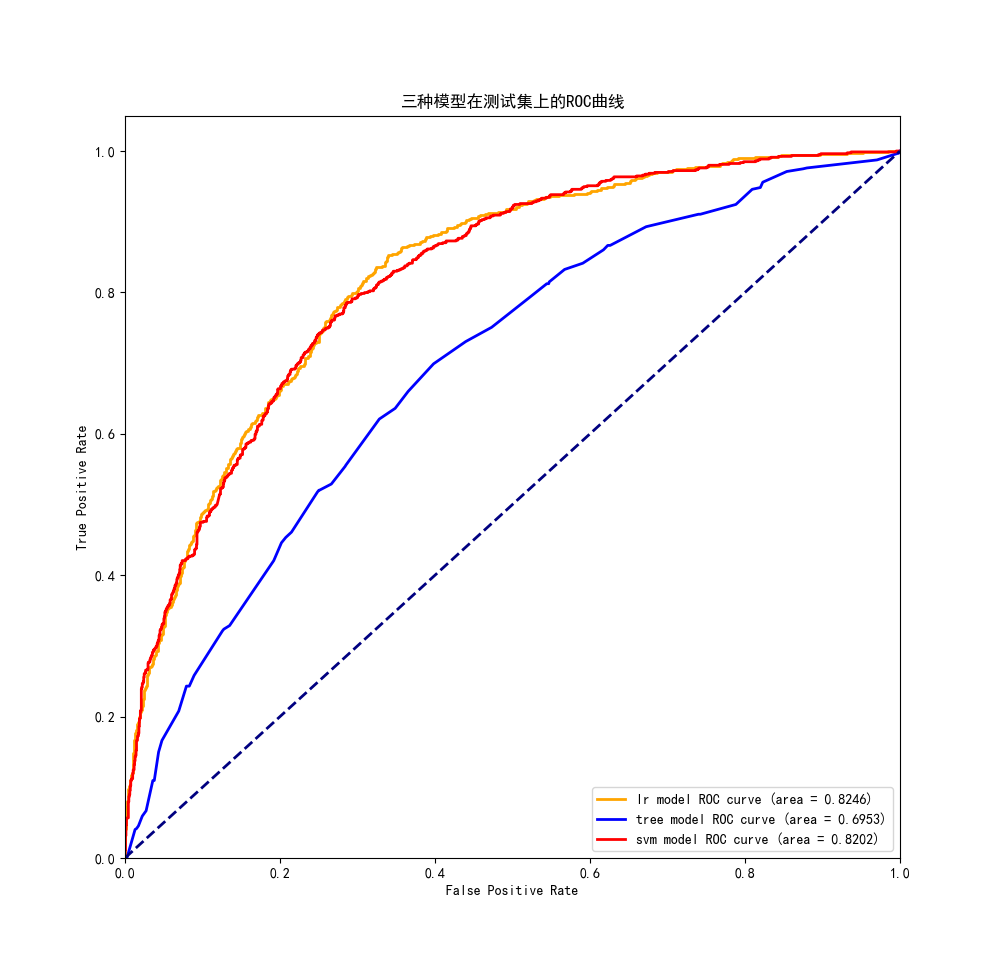
\includegraphics[width=0.9\textwidth]{ROCS.png}\\
\caption{ROCs of test set}
\label{fig:roc}
\end{figure}

$\text{注: 在实现中}tree\_clf = DecisionTreeClassifier(criterion="gini", max\_depth=6, random\_state=30)$,中决策树深度depth=6由以下最优剪枝参数学习曲线获得

\begin{figure}[H] \centering  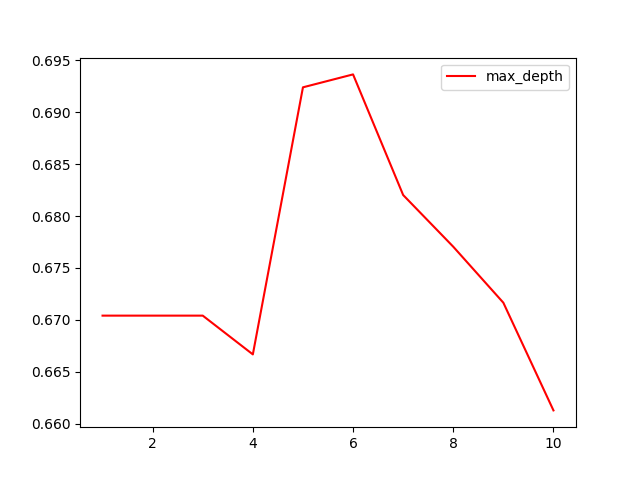
\includegraphics[scale=0.5]{确定最优剪枝参数学习曲线.png} \end{figure}

SVM的参数选择为:$svm\_clf = svm.SVC(gamma="scale", C=1.0, kernel="rbf", probability=True)$
\end{solution}



\end{document}